\documentclass[twocolumn]{aastex63}


\newcommand{\vdag}{(v)^\dagger}
\newcommand\aastex{AAS\TeX}
\newcommand\latex{La\TeX}
\usepackage{float}

% \received{June 1, 2019}
% \revised{January 10, 2019}
\accepted{May 6, 2020}
%% Command to document which AAS Journal the manuscript was submitted to.
%% Adds "Submitted to " the argument.
\submitjournal{AJ}

\shorttitle{Final Report}
\shortauthors{Hauch}


\begin{document}

\title{Visualization of Local Group Merger from M31\\From the Perspective of a Particle Within the System}
\author{Colin Hauch}

\keywords{Local Group, Galaxy Merger, Velocity dispersion, Gravitationally Bound, Stellar Disk}

\begin{abstract}
    We created a visualization of the local group merger from the perspective of a particle within the disk of the Andromeda galaxy. Visualizations are critical to providing an intuitive understanding of a dynamic system. Specifically, we explored what the sky would look like from a perspective within the system over the course of the entire simulation of the local group merger. The ability to accurately create visualizations of a specific particle is a powerful tool for lending a visual intuition to a viewer and the protocol used to create these visualizations can be used on any particle of interest. We found that almost no understanding can be gained from following a particle that moves significantly in relation to its surroundings, such as a particle within the disk of the Andromeda galaxy. This result lead us to the conclusion that a much better approach is to utilize a point within the galaxy that does not move significantly with respect to its surroundings between individual time steps, such as the center of mass of the galaxy.
\end{abstract}{}

\section{Introduction} \label{sec:intro}

We currently understand that the three largest galaxies in the local group will likely collide in the future \citep[e.g.]{vdm12,vdm19}. The local group is the largest gravitationally bound system (a system in which the gravitational force is the dominant force) that includes us.
Some publications document visualizations \citep{cox08}. There seem to be a lack visualizations created from the perspective of a planet in an M31 solar system that is in a sun-like position within M31 (8 kpc from the center of the galaxy). This is what we set out to create.

Galaxy visualizations provide a sense of visual intuition as well as give us a higher level of understanding of how internal dynamics of a galactic system are influenced by interaction. For clarity, a ``galaxy" is a collection of gravitationally bound stars whose properties can not fully be described by combination of baryons and Newton's laws of gravity \citep{will12}. 

Understanding the internal morphological change of stellar distributions within a galaxy is fundamental to our understanding of galaxies on a more foundational level and visualizations are critical to that understanding as a visually intuitive tool. These visualizations have, in the past, been from a theoretical onlooker's point of view usually at some point far from the local group itself (see Figure \ref{fig:2dvis}). This yields a field of view that can encapsulate the entire collision. We took a different approach: our view point was contained within one of the galaxies. The purpose of this approach is to create a visualization that attempts to show the sky from the perspective of a particle within the merger.

\begin{figure}
    \centering
    \includegraphics[width=3.4in]{figures/2dvis.png}
    \caption{A figure from \cite{2dvis}. This is an example of a visualization of the Milky Way from two perspectives, each being from a single point far from the center of mass of the system. The above plots show a model of the Milky Way with the three components (disk, bulge, and halo) plotted in differing colors. The axis of these plots is 100kpc. This is a great example of two-dimensional visualization that yields some level of intuition about the physical state of the system.}
    \label{fig:2dvis}
\end{figure}

Visualizations of the sky are a tricky thing to attempt to show. The sky can essentially be represented as concentric spherical shell that all the stars visible from the planet placed at some point on this shell. Plots of the sky usually manifest in a two-dimensional form which requires the utilization of some sort of mapping between a three-dimensional system (spherical shell) to a two-dimensional one (a screen or piece of paper). So, to show a three-dimensional structure in two-dimensions a ``map projection" is used. There are several of these map projections and one choice is the Mollweide Projection. A root-mean-square logarithmic distance error ($\sigma$) is often used to quantify the errors in these projections and the Mollweide projection has $\sigma = 0.39$ \citep{gott2006}. For reference, the Mercator projection has $\sigma = 0.444$ and one of the best projections, the Gott-Mugnolo azimuthal projection \citep{gott2006}, has $\sigma = 0.341$. The aim of this project is to create an intuitive medium to visually understand the local group merger via a point within the merger, using a Mollweide projection.

What would the sky look like from the perspective of a particle within one of these galaxies over the course of the merger? This is the question we are attempting to answer. 

\section{This Project} \label{sec:style}

In this paper, we will document the process of visualization of the galaxy merger (the collision of galaxies) between three galaxies for which we have the most detailed and accurate initial conditions: The Milky Way (MW), The Andromeda Galaxy (M31), and The Large Magellanic Cloud (M33). We will attempt to produce a visualization of the local group merger from the perspective of a sun-like particle within the disk of M31. 

This specifically addresses the question of what the sky would look like over the course of the local group merger from the perspective of a particle within M31. 

Understanding the morphological changes within a galaxy is essentially understanding galactic evolution. Visualizations can help us get closer to fully understanding this evolution. Creating visualizations of what the sky will look like from a particular particle would be advantageous if there was a particular interest in that particular particle. One particle that we tend to have a vested interest in is our Sun and these visualizations are a way of better understanding the dynamics of the galactic system from any perspective of any particle. 


\section{Methodology} \label{sec:style}

The paper \cite{vdm12} laid the groundwork for this visualization. They conducted an N-body simulation of the local group merger -- a simulation of a dynamical system of N particles under the influence of physical laws. They created the data set to be visualized in this project. The procedure of creating the visualization starts with choosing a set of particles.

Select a few particles that could be considered "earth like" from within the stellar bulge (particles closely packed near the center of spiral galaxies) and stellar disk (stars within a galaxy not included in the stellar bulge) and map their paths over the entire data set (perhaps relative to the center of mass of the entire system). Then, select one (or a few) of these particles as the perspective point for the visualization. Create an image (frame) of the Mollweide projection from that point via a series of coordinate transformations, each frame corresponding to a specific snap number. Do this for a series of frames and incorporate these frames into a single movie. See Figure \ref{fig:exIM} for an example frame.
\begin{figure}
    \centering
    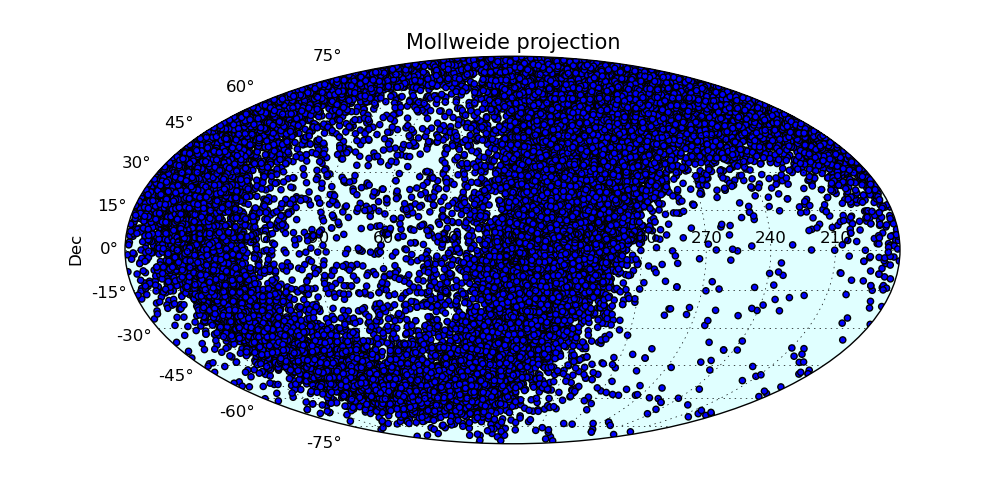
\includegraphics[width=3in]{figures/m31_DISK_from30.png}
    \caption{An example of a single frame from the perspective of one of the M31 disk particles of the other M31 disk particles on a Mollweide projection plot. Over the course of the visualization, sequential frames will presented in rapid succession giving the viewer an understanding of how the sky would change over time.  Latitude is labeled along the left edge of the image in degrees and longitude is labeled along the equator in degrees. Each point represents a particle from the M31 disk.}
    \label{fig:exIM}
\end{figure}

Many calculations must be done to make this visualization possible as well as useful. For each particle ``in the sky" of the view point particle, the displacement vector must be calculated.

$$n_{s} = n_{i}-n_{p}$$


Where $n$ represents one coordinate value in three dimensions (x,y, or z), $i$ represents the corresponding coordinate value of the $i$th particle and $p$ is the corresponding coordinate value of the perspective particle. From the displacement vector, we can perform a coordinate transformation to geographic coordinate system (latitude and longitude) via the following equations:

$$\Phi = arctan \Bigg( \frac{z}{\sqrt{x^2+y^2}} \Bigg) $$

$$\lambda = arctan \Big(\frac{y}{x}\Bigg) $$

Where $\Phi$ is the latitude, $\lambda$ is the longitude, and $x,y,z$ are the corresponding values for the displacement vector. The value for the longitude will be adjusted to account for the four combinations positive and negative $x$ and $y$ coordinates to arrive at accurate values.

The latitude and longitude coordinates can be plotted easily in a Mollweide projection (See Figure \ref{fig:exIM} for an example Mollweide projection). This would be done for all particles to be plotted. However, it is important to note that there may be too many total particles to make a useful frame. This could be solved a number of ways, one of which is by not plotting individual particles but creating a two-dimensional histogram of the sky. This would completely bypass the issue of plotting too many points which would overwhelm the viewer and ultimately lead to confusion and little to no information conveyed. 
The Mollweide projection plot is the primary plot for this paper. It is an equal-area, pseudocylindrical map projection that attempts to plot spherical coordinates as geographic coordinates.
We expect to create a visualization the provides some sense of spacial intuition for the collision of the local group. Gaining some kind of intuition for the nature of the merger could shine light on the system as a whole and inspire those to approach the research of this incredible merger event from a more well-informed position.


\section{Results} \label{sec:style}

We generated a very large number of plots over the course of this project. The first set of data utilized a sun-like particle (8kpc from the center of the galaxy) from the disk of M31 as the view point particle (VPP). A series of sequential plots can be seen in Figure \ref{fig:confusing}. 

We also generated images using a differing viewpoint: the center of mass of M31, see Figure \ref{fig:easy}. 

Videos of each of sequential frames can be found \href{https://www.youtube.com/playlist?list=PLa9bqRCotJq_bLtAAE6boyK872UA3x6rw}{here}.

% .

\section{Discussion} \label{sec:style}

As a whole, the visualization from the perspective of a single particle within M31 is absolutely not intuitive in any way whatsoever. It seems to be completely disorienting and gives the viewer almost no intuitive information about the system. This is due to the fact that the view point particle is revolving around the center of M31 (and later the center of mass of the remnant). Because the viewpoint particle moves so erratically over the course of the merger, each snap number's sky image is not necessarily similar to the last. This leads to a hopelessly disorienting and confusing series of plots (see Figure \ref{fig:confusing}). 

The effect of a view point particle moving significantly relative to its surroundings is less apparent at small snap numbers, see Figure \ref{fig:confusing}a,b,c. These sequential plots are vaguely similar and yield some understanding of the dynamics of the system. The effect is much more apparent at larger snap numbers, see Figure \ref{fig:confusing}e,f,g. At larger snap numbers sequential images are radically dissimilar, an intuition about the nature of the system is a struggle to extract. 

However, we decided to pick a point that does not move so erratically over the course of the merger as an exercise: the center of mass of the M31. This wasn't a specific particle, but does provide a significantly more intuitive understanding of the dynamics of the system. Choosing a view point that does not significantly change position relative to many of the other particles yields a much more intuitive series of plots (see Figure \ref{fig:easy}).

\section{Conclusion} \label{sec:style}

We created a visualization of the local group merger from the perspective of a particle within the disk of the Andromeda galaxy. Visualizations are critical to providing an intuitive understanding of a dynamic system. Specifically, we explored what the sky would look like from a perspective within the system over the course of the entire simulation of the local group merger. The ability to accurately create visualizations of a specific particle is a powerful tool for lending a visual intuition to a viewer and the protocol used to create these visualizations can be used on any particle of interest.

We found that using a particle within the system as a view point does not yield a visualization that makes visual sense to the viewer, as the particle moves significantly between frames relative to it's surroundings. This completely disagreed with our hypothesis that a visualization could be made with this data set using the aforementioned approach. 

However, we believe that a data set that is significantly more temporally dense would yield result that would make for more intuitive visualizations. Essentially, we believe that data sets where the view point particle does not move significantly in relation to its surroundings would produce visualizations that would indeed provide the intuition that we were initially striving for. 

\section{Acknowledgements} \label{sec:style}
We would like to thank Dr. Gurtina Belsa for the invaluable support she provided over the course of this project. We would also like to acknowledge the software that was used to facilitate the creation of this project.


Software used:

\vspace{5mm}
Astropy (Astropy Collaboration et al. 2013; Price-Whelan et al. 2018 doi: 10.3847 / 1538- 3881 / aabc4f)

matplotlib Hunter (2007),DOI: 10.1109/MCSE.2007.55

numpy van der Walt et al. (2011), DOI : 10.1109/MCSE.2011.37

FFmpeg version 4.2.2, the FFmpeg developers


\begin{figure}[p]
\gridline{\fig{Plots/000.png}{0.3\textwidth}{(a)}
          \fig{Plots/001.png}{0.3\textwidth}{(b)}
          \fig{Plots/002.png}{0.3\textwidth}{(c)}}
\gridline{\fig{Plots/474.png}{0.3\textwidth}{(d)}
          \fig{Plots/475.png}{0.3\textwidth}{(e)}
          \fig{Plots/476.png}{0.3\textwidth}{(f)}}
\caption{Plots created while using a selected particle as the view point. Each plot represents the sky from the perspective of the view point particle, shown as a Mollweide Projection. The color represents two-dimensional histogram of the total number of particles in the corresponding part of the sky (logarithmically scaled). Since there are huge fluctuations of the maximum number of particles in a particular bin over the course of the visualization, each snap number plot is scaled individually. "VVP" refers to the index of the particle within the low resolution M31 data set that was used as the view point particle. Latitude is labeled along the left edge of the image in degrees and longitude is labeled along the equator in degrees.}
\label{fig:confusing}
\end{figure}


\begin{figure}[p]
\gridline{\fig{GoodPlots/342.png}{0.3\textwidth}{(a)}
          \fig{GoodPlots/343.png}{0.3\textwidth}{(b)}
          \fig{GoodPlots/344.png}{0.3\textwidth}{(c)}}
\caption{These plots are identical to those in Figure \ref{fig:confusing} except that they do not use a single particle of the simulation as a view point. These plots are using the center of mass of M31 disk particles as the view point. This yields a much more intuitive understanding of the dynamics of the system as all sequential frames are predominately similar, especially at larger snap numbers. }
\label{fig:easy}
\end{figure}

\begin{figure}[p]
\gridline{\fig{GoodPlots/407.png}{0.3\textwidth}{(a)}
          \fig{GoodPlots/407.png}{0.3\textwidth}{(b)}
          \fig{GoodPlots/409.png}{0.3\textwidth}{(c)}}
\gridline{\fig{GoodPlots/410.png}{0.3\textwidth}{(d)}
          \fig{GoodPlots/411.png}{0.3\textwidth}{(e)}
          \fig{GoodPlots/412.png}{0.3\textwidth}{(f)}}
\caption{Additional examples of frames from the context described in Figure \ref{fig:easy}. Sequential frames from snap 407 to 412.}
\label{fig:moreEasy}
\end{figure}





% \begin{figure}
%     \centering
%     \includegraphics[height=2in]{Plots/000.png}
%     \caption{Using a Mollweide Projection, an image of the sky from the the VPP at snap = 000. Latitude is labeled along the left edge of the image in degrees and longitude is labeled along the equator in degrees. The color represents two-dimensional histogram of the total number of particles in the corresponding part of the sky (logarithmically scaled). Since there are huge fluctuations of the maximum number of particles in a particular bin over the course of the visualization, each snap number plot is scaled individually. "VVP" refers to the index of the particle used as the view point particle. This applies to each figure.}
%     \label{fig:000}
% \end{figure}

% \begin{figure}
%     \centering
%     \includegraphics[height=2in]{Plots/001.png}
%     \caption{Snap number 001}
%     \label{fig:001}
% \end{figure}{}

% \begin{figure}
%     \centering
%     \includegraphics[height=2in]{Plots/002.png}
%     \caption{Snap number 002}
%     \label{fig:002}
% \end{figure}{}

% \begin{figure}
%     \centering
%     \includegraphics[height=2in]{Plots/474.png}
%     \caption{Snap number 474; much later in the visualization. It is easy to see how an intuitive sense of the dynamics of the merger are not discernible from some sets sequential images.}
%     \label{fig:474}
% \end{figure}{}

% \begin{figure}
%     \centering
%     \includegraphics[height=2in]{Plots/475.png}
%     \caption{Snap number 475}
%     \label{fig:475}
% \end{figure}{}

% \begin{figure}
%     \centering
%     \includegraphics[height=2in]{Plots/476.png}
%     \caption{Snap number 476}
%     \label{fig:476}
% \end{figure}{}

% \begin{figure}
%     \centering
%     \includegraphics[height=2in]{GoodPlots/342.png}
%     \caption{Snap number 342 when using the center of mass of M31 as the view point. This view point seems to yield a more comprehendable series of plots.}
%     \label{fig:342}
% \end{figure}{}

% \begin{figure}
%     \centering
%     \includegraphics[height=2in]{GoodPlots/343.png}
%     \caption{Snap number 343}
%     \label{fig:343}
% \end{figure}{}

% \begin{figure}
%     \centering
%     \includegraphics[height=2in]{GoodPlots/344.png}
%     \caption{Snap number 344}
%     \label{fig:344}
% \end{figure}{}



\bibliography{demo}{}
\bibliographystyle{aasjournal}

\end{document}
